\section{Auswertung}
\label{sec:Auswertung}
  \subsection{Winkelrichtgröße}
  Die gemessene Kraft in Abhängigkeit vom dem Auslenkungswinkel wird in der Tabelle \ref{tab:tabelle1} dargestellt.
  Mit der Formel $\frac{r\cdot F}{\varphi}$ wird D berechnet.
  Mithilfe der gemessen Werte für $F$ und $\varphi$ kann mit $r = 20 \, \unit{\centi\meter}$ nun D bestimmt werden.
  Die einzelnen Werte von D sind ebenfalls in \ref{tab:tabelle1} eingetragen. 
  Mit $\overline{A} = \frac{1}{n} \sum_{i = 1}^{n} a_i$ wird nun das arithmetische Mittel gebildet. %% Brauch noch ne Quelle fürs Mittel
  Einsetzen der Werte für D und $n = 11$ ergibt $\overline{D} = 0.02 \, \unit{\newton\meter}$.

  \begin{table}
    \centering
    \caption{Tabelle 1}
    \label{tab:tabelle1}
   %% \sisetup{table-format=1.3, per-mode=reciprocal}
    \begin{tblr}{
       %% colspec = {S[table-format=3.0] S[table-format=2.1] S},
       colspec={S[table-format=2.0] S[table-format=2.0] S[table-format=2.0]},
        row{1} = {guard, mode=math},
      %%  vline{4} = {2}{-}{text=\clap{$\pm$}},
      }
      \toprule
      F \mathbin{/} \unit{\newton} & \varphi \mathbin{/} \unit{\degree} & \SetCell[c=2]{c} \symbf{D} \mathbin{/} \unit{\newton\meter} & \\
      \midrule
      0.016 &  20 & 0.009\\
      0.046 &  30 & 0.018\\
      0.066 &  40 & 0.019\\
      0.089 &  50 & 0.020\\ 
      0.11  &  60 & 0.021\\
      0.134 &  70 & 0.022\\
      0.162 &  80 & 0.023\\
      0.176 &  90 & 0.022\\
      0.18  & 100 & 0.021\\
      0.2   & 110 & 0.021\\
      0.23  & 120 & 0.022\\
      \bottomrule
    \end{tblr}
  \end{table}
    %% Siehe \autoref{fig:plot} und \autoref{tab:tabelle}!

  
  \subsection{Eigenträgheitsmoment}
  In \ref{tab:tabelle2} wird das quadrat des Abstandes der Gewichte von der Drehachse zu dem Quadrat der Schwingungsdauer aufgetragen.

  \begin{table}
    \centering
    \caption{Messwerte}
    \label{tab:tabelle2}
    \sisetup{table-format=1.2}
    \begin{tblr}{
        colspec={S S[table-format=1.0]},
        row{1}={guard, mode=math},
        }
        \toprule
        a^2/\unit{\centi\meter} & T^2/\unit{\seconds} \\ %in centimeter geändert
        \midrule     
        2.5  & 12.75\\
        5    & 13.84\\
        7.5  & 15.69\\
        10   & 18.03\\
        15   & 23.54\\
        20   & 29.81\\
        22.5 & 32.53\\
        25   & 35.84\\
        27.5 & 38.87\\
        30   & 41.81\\
        \bottomrule
    \end{tblr}
  \end{table}

  Durch das Verhältnis kann das Eigenträgheitsmoment der Drillachse bestimmt werden. 
  In \ref{fig:plot} wird T^2 zu a^2 aufgetragen.
  Mithilfe von linearer Regression wird das Verhältnis hier aufgezeigt.
  Die Steigung der Geraden enstspricht dem Eigenträgheitsmoment.
  Der Wert beträgt $I_D=717.69\unit{\kilo\gram\square\meter}$.

  \begin{figure}
    \centering
    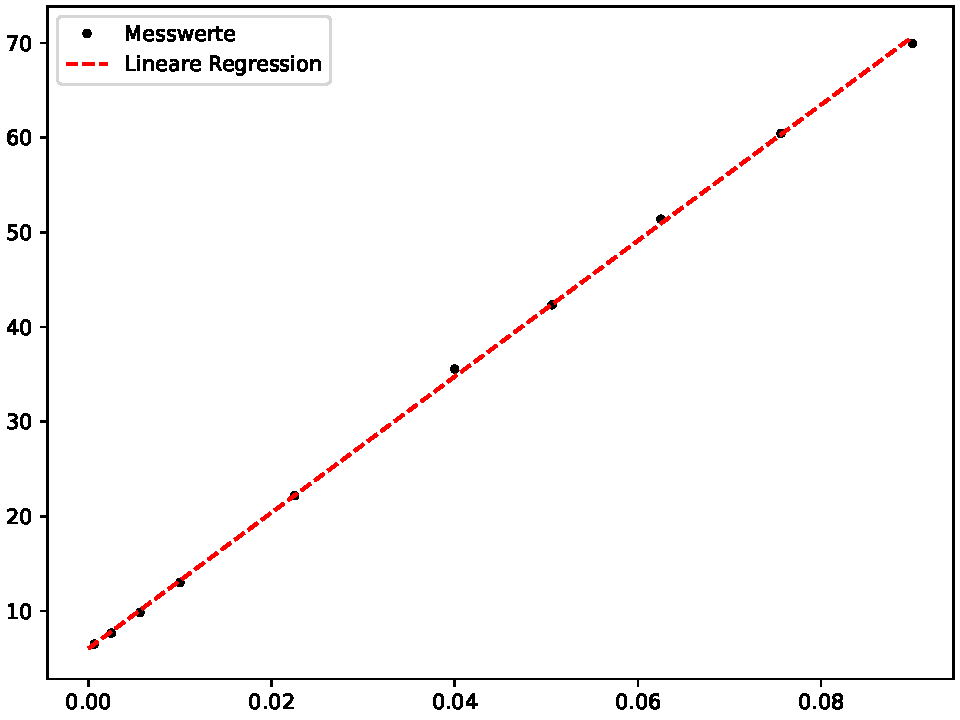
\includegraphics{plot.pdf}
    \caption{Plot.}
    \label{fig:plot}
  \end{figure}



